\newpage
\section{Performance prediction}
To answer the second research question; \textit{Is it possible to create an extensive data profile to estimate performance on
unseen datasets?}; the results from the experiments as described in \autoref{sec:performanceprediction} will be showed in this section. 

\paragraph{Strategies to estimate} The goal is to predict the performance scores (recall, precision \& F1-score) for all datasets and strategies available. But, not all strategies were able to produce results that are meaningful enough to estimate. From all the executed strategies, only strategies with an average F1-score for all datasets over 0 will be kept. As the estimation of performance results can only be done by learning from training examples, a certain amount of training samples is necessary to generate and test the estimations. Only strategies that generated results for more than 10 datasets (at least 75\% of the datasets), will be discarded for the next steps of the research. Also, for Raha, only the strategies with fully accurate human labeling simulation are taken into account. The remaining number of strategies per tool are shown in \autoref{tab:num_configs_per_tool_filtered}. In total, there are 1157 dataset-strategy pairs that will be used as input and output for training and testing. 

\begin{table}[h]
\centering
\begin{tabular}{lr}
\toprule
Tool         &  \# of configurations \\
\midrule
dBoost            &    60 \\
Raha              &    20 \\
ForbiddenItemSets &     7 \\
FAHES             &     3 \\
KATARA            &     2 \\
ActiveClean       &     1 \\
\bottomrule
\end{tabular}
\caption{Number of configurations per tool filtered with \\F1-score > 0 and at least 75\% completion}
\label{tab:num_configs_per_tool_filtered}
\end{table}

\paragraph{Estimation pipeline selection} As discussed in \autoref{subsec:estimatorselection}, an estimator pipeline will be constructed based on different regression models. The pipeline exists of four stages:
\begin{enumerate}
    \item Feature normalization/standardization (optional)
    \item Feature selection (optional)
    \item Principle component analysis (optional)
    \item Regression model (required)
\end{enumerate}

For each performance score, one estimation pipeline setting is chosen using the minimum mean square error of estimations. In each of the following subsections, the best specific estimator pipeline is discussed and the estimation results are shown. Also, the estimation errors are shown and discusses, to understand how the estimator performs.

\subsection{Precision estimation}
For the precision estimation, the best scoring estimation pipeline was:
~\\Dataset profiles $\rightarrow$ Feature normalization $\rightarrow$ Gradient Boosting Regressor
\\No principle component analysis or feature selection was done. 

~\\In \autoref{fig:prec_estimation_errors}, the distribution of estimation errors for the precision is shown. Each count represents a single estimation of the precision of a error detection strategy (tool + configuration) and a specific dataset, using the leave-one-out error. In the figure, it shows that for the precision, most of the estimations are slightly over the real values. The peak is just over 0. The median for the estimation errors is 0.0046 and the mean is -0.0092. This shows that overall, more precision estimates are over-estimations, but some of the worse estimations are underestimations (negative values). 
~\\The mean square error is 0.0537 and the median absolute error is 0.0946. This means that for most of the strategy-dataset pairs, it was capable of estimating the precision within an error of 0.1. 

\begin{figure}[h]
    \centering
    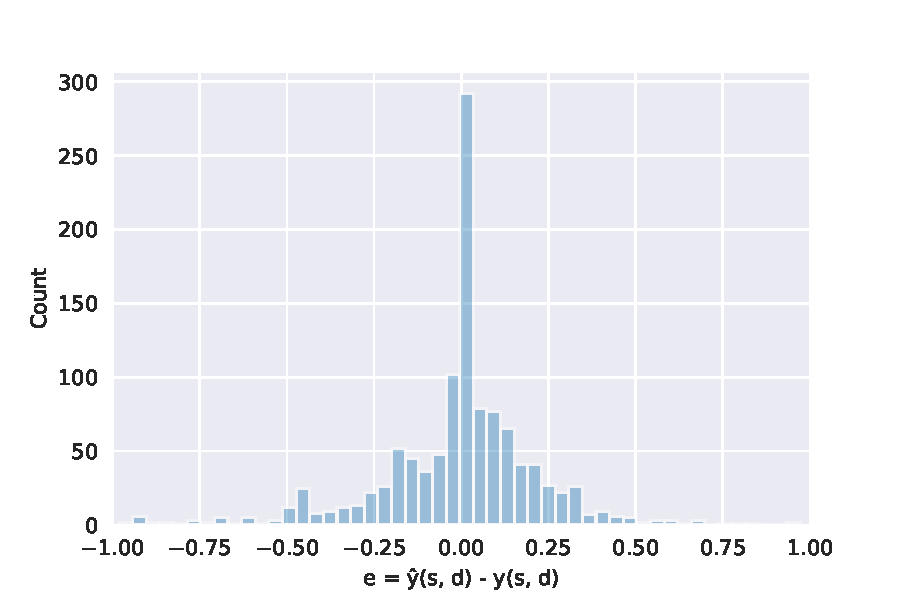
\includegraphics[width=0.75\textwidth]{thesis/Figures/RQ2/15_error_histogramcell_prec.pdf}
    \caption{Precision estimation errors distribution}
    \label{fig:prec_estimation_errors}
\end{figure}

To put these scores in perspective, if all an example random estimator would only output 0.5 as estimated precision, the mean square error would be 0.1646 and the absolute median error would be 0.45. Whereas for the selected estimator above, the estimations would make sense, having an error of around 0.45 would not provide any beneficial information before running an error detection strategy. 

\subsection{Recall estimation}
For the recall estimation, the best scoring estimation pipeline was:
~\\Dataset profiles $\rightarrow$ Select best 2 features $\rightarrow$ 3 nearest neighbours regression
\\No principle component analysis was done. 

~\\In \autoref{fig:rec_estimation_errors}, the distribution of estimation errors for the recall is shown. The best estimator pipeline for estimating the recall performs worse than it does for the precision. A mean square error 0.1045 and mean absolute error of 0.166 is achieved. The lower estimation performance can be caused by the distribution of real recall performance scores. There are around 70 dataset-strategy pairs scoring between 0 and 0.1, and approximately 300 between 0.9 and 1. Because a high recall can be achieved by marking all the cells as erroneous, this spike in the high recall score is bigger than it is with the precision estimation (around 600 between 0 and 0.1 and 50 between 0.9 and 1). Because it is easier to achieve high recall (at the cost of precision), the specific might not determine the recall of an error detection strategy as much, so it might be harder to train an estimator.

\begin{figure}[h]
    \centering
    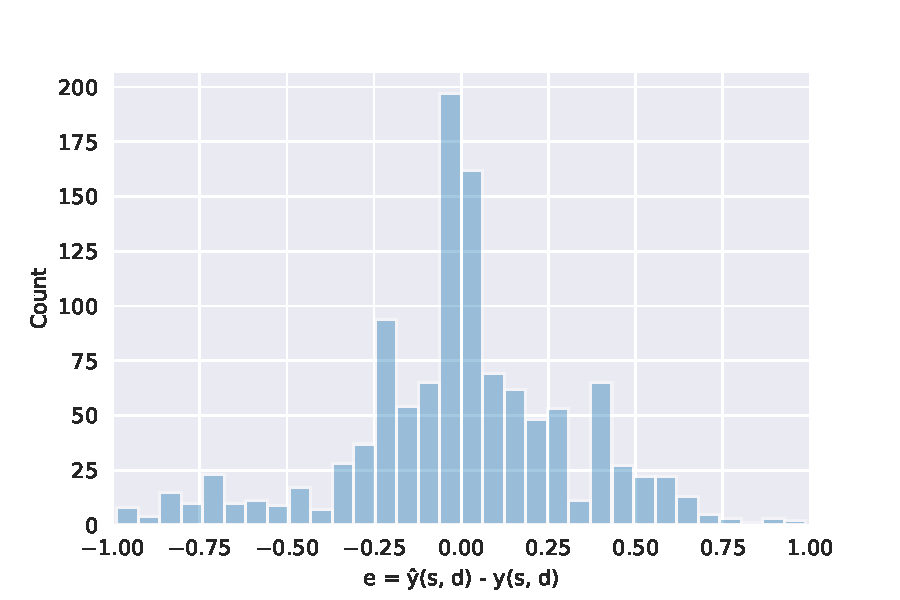
\includegraphics[width=0.75\textwidth]{thesis/Figures/RQ2/15_error_histogramcell_rec.pdf}
    \caption{Recall estimation errors distribution}
    \label{fig:rec_estimation_errors}
\end{figure}

\subsection{F1-score estimation}
% Direct vs combined
\subsubsection{Direct estimation}
For the direct F1 estimation, the best scoring estimation pipeline was:
~\\Dataset profiles $\rightarrow$ Feature standardization $\rightarrow$ PCA with RBF-kernel to 2 dimensions $\rightarrow$ Support Vector Regression

The errors of estimation are displayed in \autoref{fig:f1_estimation_errors}. With a mean square error of 0.0442 and median absolute error of 0.1006, this estimator is performing generally the best of the presented estimators, with respect to the mean square error. This best estimator for directly estimating the F1 score is mostly over-estimating values with small error margin.  

\begin{figure}[H]
    \centering
    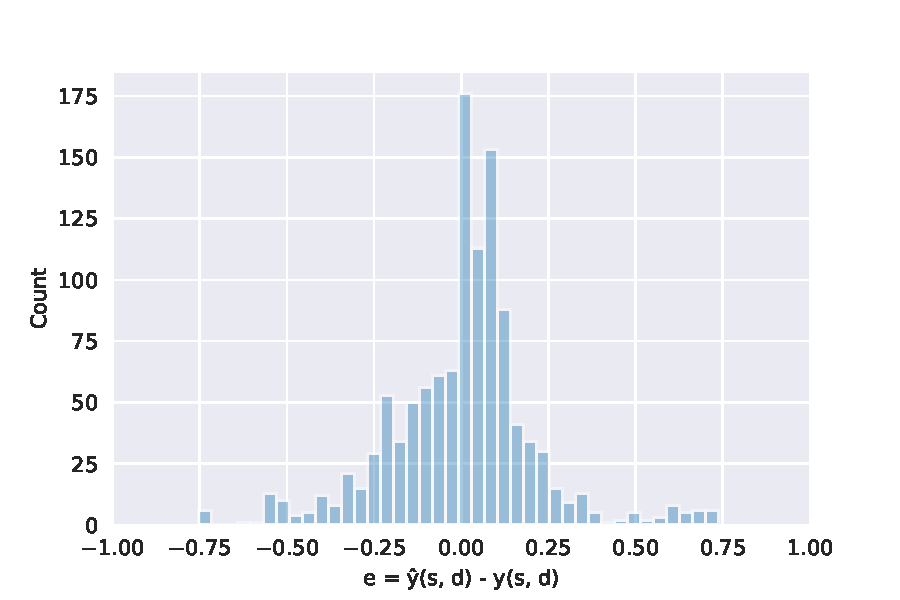
\includegraphics[width=0.75\textwidth]{thesis/Figures/RQ2/15_error_histogramcell_f1.pdf}
    \caption{F1 estimation errors distribution}
    \label{fig:f1_estimation_errors}
\end{figure}

\subsubsection{Combined estimation}
The combined estimator is the using the best estimator pipelines from the precision and recall together to output an F1-score. The error distribution is shown in \autoref{fig:combined_f1_estimation_errors}. The main noticeable finding is that the distribution shifted more towards the center, performing better in general than the direct F1 score estimator. With a median absolute error of only 0.0762, it outperforms the direct estimator for most of the samples, but due to the under-estimated outliers on the left of \autoref{fig:combined_f1_estimation_errors}, the mean square error is neglectably higher (0.0449). 

\begin{figure}[h]
    \centering
    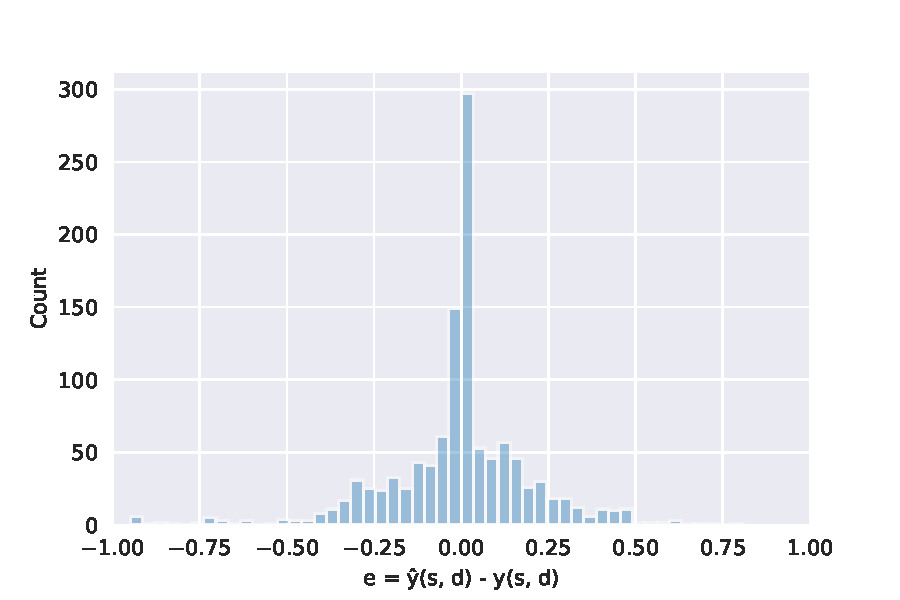
\includegraphics[width=0.75\textwidth]{thesis/Figures/RQ2/15_error_histogramcell_f1_combined.pdf}
    \caption{Combined F1 estimation errors distribution}
    \label{fig:combined_f1_estimation_errors}
\end{figure}

\subsection{Results per tool}
To verify how the specific estimators perform for each tool, the mean squared error grouped for each tool is shown in \autoref{fig:mse_combined_f1_tool}. It shows that for Raha, the best performing tool, has the highest mean square error. ActiveClean follows in the highest error. This could imply that it is harder to estimate error detection strategies with a human in the loop. Also, both Raha and ActiveClean are based on partially random sampling for the human labeling, which could give different results for different runs. Lastly, the fact that Raha performs best overall, also contributes to possible over-estimations for a dataset like "restaurants", where no tool performed better than 0.01 F1-score. 

\begin{figure}[H]
    \centering
    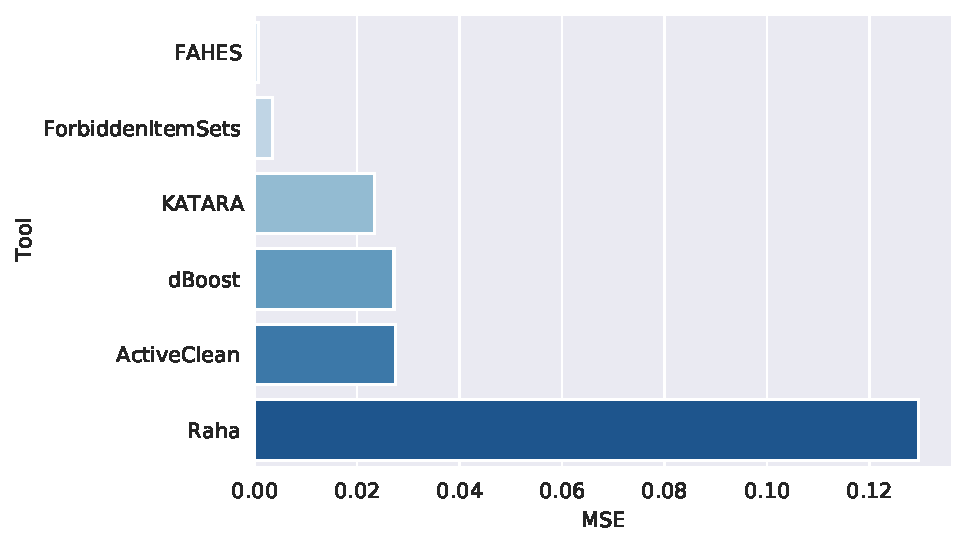
\includegraphics[width=0.8\textwidth]{thesis/Figures/RQ2/15_tools_combined_f1.pdf}
    \caption{Mean squared error for combined F1 estimation, grouped on tool}
    \label{fig:mse_combined_f1_tool}
\end{figure}


\subsection{Evaluation}
% Qualitatively
Qualitatively, the error distributions in the section above meet the criteria set in \autoref{subsec:evaluation_performanceprediction}. The distributions are heavily centered around 0, indicating that most estimations are close to perfect. Also the distributions are cleary non-uniform. Only the recall estimation shows larger clusters of outliers, but combined with the precision estimation, it gives a promising output without clusters of errors for the combined F1 estimation as seen in \autoref{fig:combined_f1_estimation_errors}. For comparison, the error estimation distribution of the combined F1 baseline estimation is shown in \autoref{fig:baseline_combined_f1_estimation_errors}. This clearly shows that the proposed estimator has an improved error distribution (\autoref{fig:combined_f1_estimation_errors}) over the baseline, which is mostly overestimating. 

\begin{figure}[h]
    \centering
    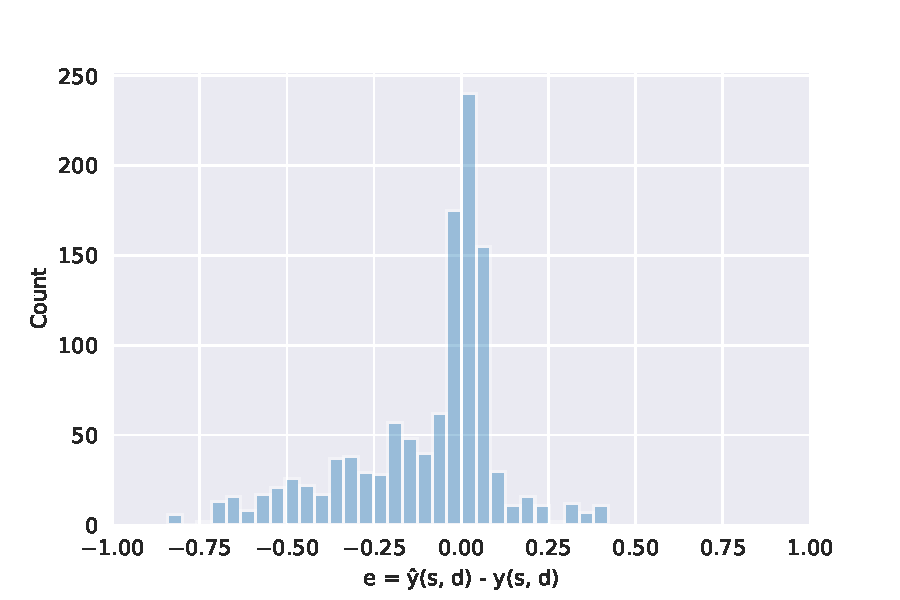
\includegraphics[width=0.75\textwidth]{thesis/Figures/RQ2/15_average_estimator_error_histogramcell_f1_combined.pdf}
    \caption{Baseline combined F1 estimation errors distribution}
    \label{fig:baseline_combined_f1_estimation_errors}
\end{figure}

% Quantitatively
In \autoref{tab:performance_estimation_comparison_baseline}, the comparison with the baseline for the mean squared error (MSE) and median absolute error (MAE) is given. For all estimation experiments, the proposed estimators score better than the baseline method. This means that it the estimator models are capable of learning information from the dataset profiles and are not just taking average scores of previously seen entries.

\begin{table}[h]
\centering
\begin{tabular}{ll|l|l}
                     &              & \textbf{Baseline} & \textbf{Estimator} \\ \hline
\textbf{Precision}   & \textbf{MSE} & 0.0598            & {\ul 0.0537}       \\ \hline
\textbf{}            & \textbf{MAE} & 0.1357            & {\ul 0.0946}       \\ \hline
\textbf{Recall}      & \textbf{MSE} & 0.1126            & {\ul 0.1045}       \\ \hline
\textbf{}            & \textbf{MAE} & 0.2084            & {\ul 0.1660}       \\ \hline
\textbf{Direct F1}   & \textbf{MSE} & 0.0484            & {\ul 0.0442}       \\ \hline
\textbf{}            & \textbf{MAE} & 0.1264            & {\ul 0.1006}       \\ \hline
\textbf{Combined F1} & \textbf{MSE} & 0.0586            & {\ul 0.0449}       \\ \hline
\textbf{}            & \textbf{MAE} & 0.0787            & {\ul 0.0762}      
\end{tabular}
\caption{Estimator model and baseline method comparison for performance prediction}
\label{tab:performance_estimation_comparison_baseline}
\end{table}

There are some limitations to these experiments. Like stated in \autoref{subsec:evaluation_empirical_study_results}, due the infeasibility of re-running experiments, all configurations were run once on each dataset. ActiveClean and Raha rely on random sampling for human labeling. This could imply that a performance estimation made by the models might be correct on historical data, but not on new tests, due to randomness. Also, there would have been repetitions in experiments, it would be unclear on which performance results (latest, best, first, etc..) or which possible aggregate of results (mean, max, min, etc..) to use for estimation. Therefore, in this stage there has been chosen to only include single experiment results.

Also, the settings of each estimator pipeline are chosen to be same for each performance metric (precision, recall and F1 separately). Another possibility would be picking the optimal setting of the estimator pipeline for each specific strategy. This could improve estimation, but also leads to more complexity and possible overfitting. It should also be taken into accoun that the minimization for finding the best estimator was done using the mean squared error, but other metrics could be fitting as well, like the mean absolute error. This would change the resulting "best" model and its estimation error distribution.

Concluding, both qualitatively and quantitatively the experiments show positive results. So, from the experimental results, it seems possible to create an extensive data profile to estimate performance on unseen datasets, with acceptable distributions of estimation errors, using the proposed estimator models. 